\documentclass[a4paper,  margin=1in]{report}
\usepackage{graphicx}
\usepackage[utf8]{inputenc}

\DeclareUnicodeCharacter{03C6}{\ensuremath{\phi}}
\DeclareUnicodeCharacter{03C0}{\ensuremath{\pi}}
\begin{document}

\Large
\begin{center}
    Rīgas Tehniskā Universitāte\\
    Elektronikas un telekomunikāciju fakultāte\\
    Radioelektronikas institūts\\
    Elektronikas pamatu katedra\\ 
    \vspace{50pt}
    \textbf{
        Signālu teorijas pamati\\
        Laboratorijas darbs Nr. 2.\\}
    \vspace{120pt}
    \textbf{
        Iepazīšanās ar periodisku signālu izvērsi\\
        trigonometrisku funkciju Furjē rindā\\
    }

    \vspace{120pt}
\end{center}
\begin{flushright}
    Andris Kučiks\\
    REBMO\\
    Stud. apl. Nr. 151REB073\\
\end{flushright}
\vspace{50pt}
\begin{center}
    RĪGA\\
    2017\\
\end{center}
\vspace{10pt}
\newpage 

\normalsize
\underline{
    Darbā izmantotā blokshēma:
}\\
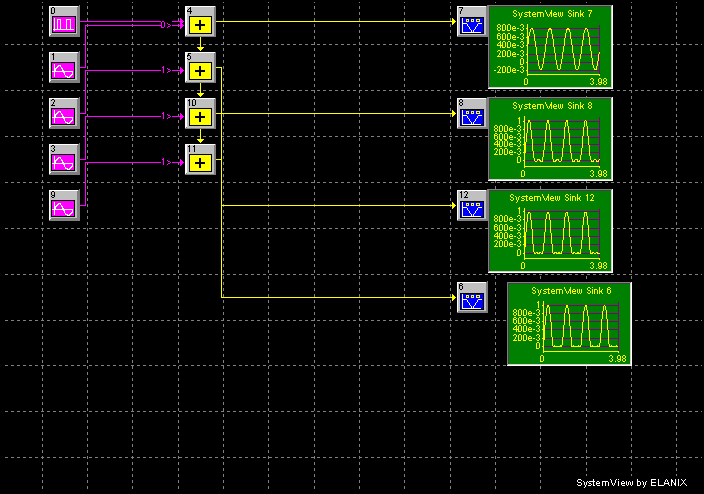
\includegraphics[width=\textwidth,height=\textheight,keepaspectratio]{v2_1.png}
Saīsinājumi: Signāla amplitūda -S a ; frekvence- f; faze-φ; nobīde – Of, Pulse Width -PW\\
\underline{Bloku parametri:}\\
0 - līdzkomponentes ģenerators S a =1/π=318.31e-3 V, f =0.1Hz, φ=0, Of=0;PW=4 sec;\\
1- sinusoidāls ģenerators S a =0.5V, f=1Hz, φ=0;\\
2- sinusoidāls ģenerators S a =-0.212V, f=2Hz, φ=0;\\
3- sinusoidāls ģenerators S a =-0.042V, f=4Hz, φ=0;\\
9- sinusoidāls ģenerators S a =-0.018V, f=6Hz, φ=0;\\
\underline{Simulēšanas laika parametri:}\\
Start Time = 0 sec;\\
Stop Time = 3.984375 sec;\\
No. of Samples = 256;\\
Sample Rate = 64Hz;\\
Time Spacing = 15.625*e-3;\\
Frequency Resolution = 250e-3 Hz.\\
\end{document}
